\RequirePackage{fix-cm} % https://dtrx.de/od/tex/sfmath.html
\documentclass{article}
\usepackage[paperwidth=5.2in, paperheight=3cm, margin=0in]{geometry}
\usepackage{tikz}
\usetikzlibrary{calc,patterns,decorations.pathmorphing,decorations.markings, positioning}
\usetikzlibrary{arrows}

\renewcommand{\familydefault}{\sfdefault}
\usepackage[]{sfmath}

%\usepackage{cmbright} %% a sans-serif font for math




\newcommand{\dotswidth}{0cm}
\newcommand{\masswidth}{1cm}
\newcommand{\massheight}{0.6cm}
\newcommand{\wallthickness}{0.25cm}
\newcommand{\figwidth}{2.7*4.1cm}
\newcommand{\springlength}{\figwidth/6-5*\masswidth/6}
\newcommand\wallspringlength{1.2cm}

\newcommand{\massonepos}{\springlength+\masswidth/2}
\newcommand{\masstwopos}{\massonepos+\masswidth+\springlength}
\newcommand{\massthreepos}{\masstwopos+\springlength+\masswidth}
\newcommand{\massfourpos}{\massthreepos+\springlength+\masswidth}
\newcommand{\massfivepos}{\massfourpos+\springlength+\masswidth}
\newcommand{\wallonepos}{\massonepos-\wallspringlength}
\newcommand{\walltwopos}{\masstwopos-\wallspringlength}
\newcommand{\wallthreepos}{\massthreepos-\wallspringlength}
\newcommand{\wallfourpos}{\massfourpos-\wallspringlength}
\newcommand{\wallfivepos}{\massfivepos-\wallspringlength}
\newcommand{\rightdotspos}{\massfivepos+\springlength+\masswidth/2}

\newcommand{\levelone}{1.2cm}  % higher level, level of walls

\newcommand{\labelheight}{-.9cm} %+.76cm
\newcommand{\wallheight}{.7cm}
\newcommand{\circlesize}{.02cm}

\begin{document}

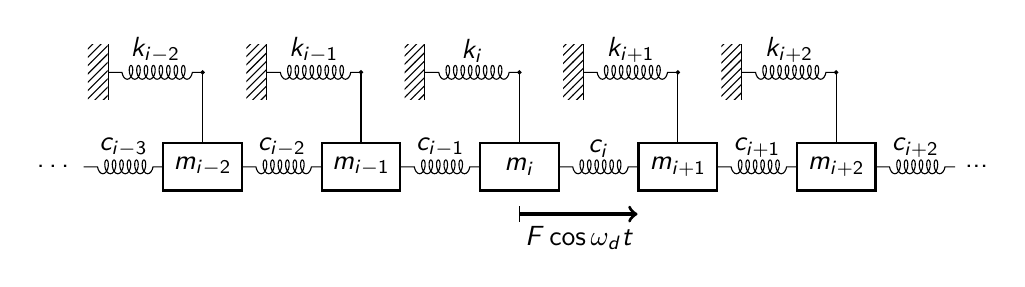
\begin{tikzpicture}[]

%% two options for spring style
%\tikzstyle{spring}=[decorate,decoration={zigzag,pre length=0.2cm,post length=0.2cm,segment length=3}]
\tikzstyle{spring}=[decorate,decoration={coil,pre length=0.13cm,post length=0.13cm,segment length=2.7}]

\tikzstyle{wall}=[fill,pattern=north east lines,draw=none,minimum width=\wallthickness,minimum height=\wallheight]


%% draw walls
%\node (rightwall)[wall, xshift =\rightdotspos,yshift=\wally,anchor=west]{};
%\draw (rightwall.north west) -- (rightwall.south west);


%% define ldots
\node (leftdots) [minimum width=\dotswidth, anchor=east] {\ldots};
%\node (rightdots)  {\ldots};

%% five masses
\node(M1)  [minimum width=\masswidth,minimum height=\massheight, xshift=\massonepos, style={draw,outer sep=0pt,thick}] {$m_{i-2}$};
\node(M2)  [minimum width=\masswidth,minimum height=\massheight, xshift =\masstwopos,style={draw,outer sep=0pt,thick}] {$m_{i-1}$};
\node(M3)  [minimum width=\masswidth,minimum height=\massheight, xshift =\massthreepos,style={draw,outer sep=0pt,thick}] {$m_{i}$};
\node(M4)  [minimum width=\masswidth,minimum height=\massheight, xshift =\massfourpos,style={draw,outer sep=0pt,thick}] {$m_{i+1}$};
\node(M5)  [minimum width=\masswidth,minimum height=\massheight, xshift =\massfivepos,style={draw,outer sep=0pt,thick}] {$m_{i+2}$};

%% vertical lines above masses
%\draw (M1.north)--(M1.north,\levelone)

%% vertical lines up to upper level
\draw [fill] circle [radius=\circlesize, xshift=\massonepos, yshift=\levelone] {};  % xshift to match m1
\draw(M1.north)--(\massonepos,\levelone);
\draw [fill] circle [radius=\circlesize, xshift=\masstwopos, yshift=\levelone] {};  % xshift to match m1
\draw(M2.north)--(\masstwopos,\levelone);
\draw [fill] circle [radius=\circlesize, xshift=\massthreepos, yshift=\levelone] {};  % xshift to match m3
\draw(M3.north)--(\massthreepos,\levelone);
\draw [fill] circle [radius=\circlesize, xshift=\massfourpos, yshift=\levelone] {};  % xshift to match m1
\draw(M4.north)--(\massfourpos,\levelone);
\draw [fill] circle [radius=\circlesize, xshift=\massfivepos, yshift=\levelone] {};  % xshift to match m1
\draw(M5.north)--(\massfivepos,\levelone);
%\draw[spring] (\massonepos,\levelone) -- (\massthreepos,\levelone);
%\node [above] at (\ktwothreepos,\levelone+.1cm) {$k_{13}$};

%% draw five walls springs, no text
%\draw[spring](\massonepos,\levelone)--(\wallonepos,\levelone)
%\draw[spring](\masstwopos,\levelone)--(\walltwopos,\levelone);
%\draw[spring](\massthreepos,\levelone)--(\wallthreepos,\levelone);
%\draw[spring](\massfourpos,\levelone)--(\wallfourpos,\levelone);
%\draw[spring](\massfivepos,\levelone)--(\wallfivepos,\levelone);

%% draw five walls springs
\draw[spring](\massonepos,\levelone)--(\wallonepos,\levelone) node[draw=none,fill=none,font=\normalsize,midway,above] {$k_{i-2}$};
\draw[spring](\masstwopos,\levelone)--(\walltwopos,\levelone) node[draw=none,fill=none,font=\normalsize,midway,above] {$k_{i-1}$};
\draw[spring](\massthreepos,\levelone)--(\wallthreepos,\levelone) node[draw=none,fill=none,font=\normalsize,midway,above] {$k_{i}$};
\draw[spring](\massfourpos,\levelone)--(\wallfourpos,\levelone) node[draw=none,fill=none,font=\normalsize,midway,above] {$k_{i+1}$};
\draw[spring](\massfivepos,\levelone)--(\wallfivepos,\levelone) node[draw=none,fill=none,font=\normalsize,midway,above] {$k_{i+2}$};



%% draw five walls (hash lines and vertical line)
\node (wallone)  [wall, xshift=\wallonepos, yshift=\levelone,anchor=east] {}; % hashline
\draw (wallone.north east) -- (wallone.south east); % vertical line
\node (walltwo)  [wall, xshift=\walltwopos, yshift=\levelone,anchor=east] {};
\draw (walltwo.north east) -- (walltwo.south east);
\node (wallthree)  [wall, xshift=\wallthreepos, yshift=\levelone,anchor=east] {};
\draw (wallthree.north east) -- (wallthree.south east);
\node (wallfour)  [wall, xshift=\wallfourpos, yshift=\levelone,anchor=east] {};
\draw (wallfour.north east) -- (wallfour.south east);
\node (wallfive)  [wall, xshift=\wallfivepos, yshift=\levelone,anchor=east] {};
\draw (wallfive.north east) -- (wallfive.south east);

%% six coupling springs  %% try using position command    at ($(M1)!.5!(M2)$)    to be halfway between
\draw[spring] (M1.west)--(\dotswidth,0)  node[draw=none,fill=none,font=\normalsize,midway,above] {$c_{i-3}$};
\draw[spring](M2.west)--(M1.east)   node[draw=none,fill=none,font=\normalsize,midway,above] {$c_{i-2}$};
\draw[spring](M3.west)--(M2.east) node[draw=none,fill=none,font=\normalsize,midway,above] {$c_{i-1}$};
\draw[spring](M4.west)--(M3.east) node[draw=none,fill=none,font=\normalsize,midway,above] {$c_{i}$};
\draw[spring](M5.west)--(M4.east) node[draw=none,fill=none,font=\normalsize,midway,above] {$c_{i+1}$};
\draw[spring](\rightdotspos,0)--(M5.east) node[draw=none,fill=none,font=\normalsize,midway,above] {$c_{i+2}$};

%% draw right elipses
\node (rightdots) [minimum width=\dotswidth,xshift = \rightdotspos, anchor=west] {$\ldots$};

%% force label
\newcommand{\arrowheight}{\labelheight+.3cm}
\newcommand{\Fcosheight}{\labelheight} % + .27 cm
\node[ anchor=west] at (\massthreepos - .05 cm,\Fcosheight) {$F \cos \omega_d t$};
\draw[very thick,->](\massthreepos,\arrowheight) --(1.5cm+\massthreepos,\arrowheight);
%\draw (M1.north)--(\massthreepos, 1 cm); % option 1
\draw (\massthreepos, \arrowheight - .1cm)--(\massthreepos, \arrowheight+.1cm); % option 2


%\draw [spring] (leftwall.east) -- (leftwall.east+1cm){k1};

\end{tikzpicture}


\end{document}